\section{Sub-atomic Particles}

\subsection{atomic structure}

\subsubsection{atomic model}\label{ch:atomic-model}

\begin{wrapfigure}{r}{0.4\textwidth}
	\vspace*{5pt}
	\centering
	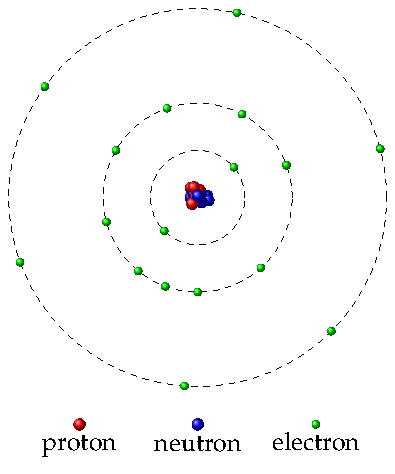
\includegraphics[height=180pt]{atomic-model}
	\vspace*{-20pt}
\end{wrapfigure}

all matter is composed of tiny particles called \keypoint{atoms}

each different element has its own type of atom

the diagram below illustrates a simple atomic model\index{atomic model}


\cmt at centre of each atom is the \keypoint{nucleus}\index{nucleus}

\cmt radius of an atom $\sim 10^{-10} \sim 10^{-9} \text{ m}$

radius of a nucleus $\sim 10^{-15} \sim 10^{-14} \text{ m}$

\cmt particles that make up a nucleus are called \keypoint{nucleons}\index{nucleon}

nucleons come in two types, \keypoint{protons} and \keypoint{neutrons}\index{proton}\index{neutron}

\cmt outside the nucleus are the \keypoint{electrons}\index{electron}

electrons move around the nucleus in a \emph{cloud}

\cmt protons, neutrons and electrons are the building blocks of all atoms and hence the building blocks for all matter

\cmt properties of protons, neutrons and electrons are listed below

\begin{compactenum}
	\item[--] charge of each proton and electron is the elementary charge unit: $e = 1.60 \times10^{-19} \text{ C}$
	
	\item[--] neutron has zero charge
	
	\item[--] a proton has very similar mass as a neutron
	
	\item[--] electron has much smaller mass than a nucleon (proton or neutron)
\end{compactenum}

\begin{center}
	\begin{tabular}{|C{3.5cm}|C{1.6cm}|C{3.5cm}|C{2.8cm}|}
		\hline subatomic particle & charge & mass & location found \\ 
		\hline proton & $+e$ & $m_p = 1.67 \times 10^{-27}$ kg & nucleus \\ 
		\hline neutron & 0 & $m_n = 1.67 \times 10^{-27}$ kg & nucleus \\ 
		\hline electron & $-e$ & $m_e = 9.11 \times 10^{-31}$ kg & in outer atom \\ 
		\hline 
	\end{tabular}
\end{center}

\subsubsection{\texorpdfstring{$\alpha$}{\textsubscript{\textalpha}}-particle scattering experiment}

experiments were designed to verify if the model gives the right description of an atom

one of the most important experiments carried out was the \keypoint{$\alpha$-particle scattering experiment}\index{$\alpha$-particle scattering experiment}

under the direction of \emph{Ernest Rutherford}, \emph{Hans Geiger} and \emph{Ernest Marsden} studied atomic structure by firing $\alpha$-particle beam towards a thin gold foil  at the University of Manchester

\begin{figure}[!ht]
	\centering
	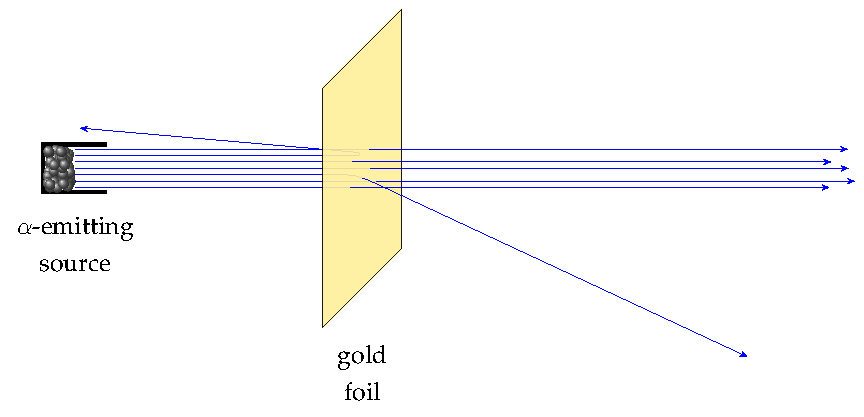
\includegraphics[height=180pt]{alpha-scattering}
	\caption*{Rutherford's $\alpha$-particle scattering experiment}
\end{figure}

\begin{figure}[!ht]
	\centering
	\begin{tikzpicture}[scale=1.33]
		\shade[ball color=Gold] (0,0) circle (.2);
		\node[right, twoline] at (0.3,0) {gold\\nucleus}; 
		\draw[blue,->] (-4,0.03) -- (-0.4, 0.03) arc(-90:86:0.04) --++ (176:2.5);
		\draw[blue,->] (-4,1) -- (3, 1);
		\draw[blue,->] (-4,-1.2) -- (3, -1.2);
		\draw[blue,->] (-4,-0.5) -- (-1,-0.5) arc(90:65:4) --++ (-25:2.4);
	\end{tikzpicture}
	
	\caption*{paths of $\alpha$-particles as they approach and pass by a gold nucleus}
\end{figure}




\cmt the main experimental results of the experiments are

\begin{compactitem}
	\item[--] most $\alpha$-particles pass straight through the foil with almost no deflection
	
	\item[--] very few $\alpha$-particles (about 1 in $10^4$) are deflected by large angles.
\end{compactitem}

\cmt to explain the observations, Rutherford concluded the following about nature of atoms

\begin{compactitem}
	\item[--] most space in an atom is empty
	
	(so most $\alpha$-particles merely pass through empty space without deflection)
	
	\item[--] there is a tiny positively-charged core, called the nucleus, at centre of an atom
	
	(so only a small fraction of $\alpha$-particles would interact with the nucleus)
	
	\item[--] almost all mass of the atom is concentrated in the nucleus
	
	(so interaction is influential if nucleus happens to sit on the path of $\alpha$-particle beam)
\end{compactitem}

based on these understandings, Rutherford proposed the atomic model introduced in \S\ref{ch:atomic-model}

this model is now known as \emph{Rutherford's model}, or \emph{planetary model of the atom}
\footnote{
	Before Ernest Rutherford, the most popular atomic model at the time was proposed by \emph{J. J. Thompson} of the Cavendish Lab at the University of Cambridge. Thompson first discovered electrons from cathode rays. He showed that electrons are negatively-charged and hence proved that an atom is made up of electrons and something that carries positive charges. He suggested that electrons are evenly distributed in a positive cloud of matter, which is now called the \emph{plum-pudding model}.
	
	To verify this model, Rutherford's group set out and designed the gold foil experiment. The plum-pudding model predicts that deflection of $\alpha$-particles should be uniformly distributed around the central beam, but there is no reason that an $\alpha$-particle would undergo a large change in its direction of motion, like a cannonball hitting a piece of paper and rebounding backwards. The results of the scattering experiment meant that the plum-pudding model had to be overturned. In order to explain the experimental observations, Rutherford then put forward the new model which now bears his name.}
\footnote{
	 Rutherford originally suggested that electrons rotate around the nucleus in \emph{circular} orbits due to attractive electrostatic force, like the planets orbit around the sun. This is why Rutherford's model of atomic structure is also called \emph{the planetary model of the atom}.
	 
	 However, later studies showed that Rutherford's model had its own problems. Classical electromagnetic theory suggests that any charged particle in accelerated motion would radiate energy, so the orbiting electrons will gradually lose all its energy and fall into the nucleus. An atom can never be stable if the Rutherford's model is correct. The full description of the atomic structure requires the understanding of the \emph{quantum} behaviour of electrons, which are described by \emph{probability waves}. Electrons actually do not move in circular orbits but have a certain probability to be anywhere in space at any time, forming an \emph{electron cloud}.
 }




\subsubsection{nuclide notation}

\keypoint{nuclides} are specific types of atoms or nuclei

a nuclide is uniquely defined by its \keypoint{proton number} $Z$ and its \keypoint{nucleon number} $A$

a nuclide is usually denoted as $\boxed{_Z^A X}$, where $X$ is the chemical symbol for the element

\cmt by definition, $Z$ gives number of protons, $A$ gives number of nucleons

as a consequence, number of neutrons is given by $N = A-Z$

\cmt proton number $Z$ can be further interpreted as \keypoint{charge number} of the particle \index{charge number}

recall each proton carries charge $+e$, and neutrons are chargeless

so $Z$ further determines electrical charge of the nucleus: $\boxed{Q = +Ze}$

this extension will be important when we deal with other particles later in this chapter

\cmt nucleon number $A$ can be interpreted as \keypoint{mass number} of the particle \index{mass number}

each proton and neutron is of approximately the same mass

so mass of nucleus is determined by total number of protons and neutrons: $\boxed{m = A\text{u}}$

where $1 \text{ u} = 1.66\times10^{-27} \text{ kg}$ is the \keypoint{unified atomic mass unit}
\footnote{Note that the unified atomic mass ($1.661\times10^{-27} \text{ kg}$), formally defined as one twelfth of the mass of an carbon-12 atom, is slightly less than the mass of a \emph{free} proton ($m_p=1.673\times10^{-27} \text{ kg}$ or that of a \emph{free} neutron ($m_n=1.675\times10^{-27} \text{ kg}$). This is because energy goes out when protons and neutrons combine to form a nucleus, and this would be associated with a decrease in the mass as suggested by \emph{Albert Einstein's mass-energy equivalence principle}. You can think of $\text{u}$ as the average mass of a proton or a neutron when a group of them squeeze together. If you want to find out the mass of a nucleus, you should use $\text{u}$. But if you are dealing with a single proton or a single neutron, you should use $m_p$ and $m_n$ instead.}

\cmt using this notation, protons, neutrons and electrons can be represented by: $ \boxed{^1_1\text{p}}$, $\boxed{^1_0\text{n}}$, $\boxed{^{\phantom{-}0}_{-1}\text{e}} $

\example{The nuclide uranium-238 can be denoted by $^{238}_{\phantom{2}92}\text{U}$. (a) State its proton number and its neutron number. (b) Find the charge and mass of the uranium-238 nucleus.}

\sol proton number: $Z=92$

neutron number: $N=A-Z=238-92=146$

nuclear charge: $Q=+Ze=+92\times1.60\times10^{-19}\approx1.47\times10^{-17}\text{ C}$

mass of nucleus: $m=A\text{u} = 238 \times 1.66\times10^{-27} \approx 3.95 \times 10^{-25}\text{ kg}$ \eoe


\example{Radius of a copper-64 nucleus is $4.8\times10^{-15} \text{ m}$. Calculate the mean nuclear density.}

\solc\begin{equation*}
	\rho = \frac{m}{V} = \frac{A\text{u}}{\frac{4}{3}\pi r^3} = \frac{64 \times 1.66\times10^{-27}}{\frac{4}{3}\pi \times (4.8x10^{-15})^3} \RA \rho \approx 2.3 \times 10^{17} \text{ kg m}^{-3}
\end{equation*}

this is much greater than density of a copper block (about $8.9 \times  10^3 \text{ kg m}^{-3}$)

we can therefore infer that the nucleus indeed takes most mass of the atom \eoe


\subsubsection{chemical properties of elements}

chemical properties of an atom depend on the number of electrons

\cmt proton number $Z$ also gives the \keypoint{atomic number} of the element

in a neutral atom, there are same number of protons as electrons

so atoms of same chemical properties, i.e., atoms of same element have same proton number

\cmt atoms of same chemical properties can have different nuclei

\keypoint{isotopes} of same element have same number of protons but different number of neutrons\index{isotope}





\example{State and explain whether carbon-12 ($^{12}_{\phantom{1}6}\text{C}$) and carbon-14  ($^{14}_{\phantom{1}6}\text{C}$) are different isotopes of the same element.}

\sol both carbon-12 and carbon-14 atoms have 6 protons

but carbon-12 has 6 neutrons, carbon-14 has 8 neutrons

same proton number but different neutron number, so different isotopes of same element \eoe




\subsection{radioactivity}

\subsubsection{radioactive decays}

if a nucleus is unstable then it may break down by releasing radiation from the nucleus

this process is called \keypoint{radioactive decay}\index{radioactive decay}

\cmt three most common types of radioactive decays are $\alpha$-decay, $\beta$-decay and $\gamma$-decay

\cmt radioactive decays are \emph{spontaneous}

decay events are independent of outside conditions, such as temperature, pressure, etc.

whether one nucleus is about to decay is also independent of the other nuclei around it

radioactive decays only depend on the internal stability of the nucleus

\cmt radioactive decays are \emph{random}

one cannot predict when and which nucleus will decay

an unstable nucleus might decay at any time

whether or not decay occurs can only be given by probabilities





\subsubsection{properties of \texorpdfstring{$\alpha$}{\textsubscript{\textalpha}}-, \texorpdfstring{$\beta$}{\textsubscript{\textbeta}}- \& \texorpdfstring{$\gamma$}{\textsubscript{\textgamma}}-radiation}

\subsubsection*{nature of \texorpdfstring{$\alpha$}{\textalpha}-radiation}

$\alpha$-particles are \emph{helium nuclei}, each made up of two protons and two neutrons\index{radioactive decay!$\alpha$-decay}

an $\alpha$-particle therefore carries a positive charge of 2$e$, and a mass of 4u

$\alpha$-particles emitted from a given source travel at almost the same speed

speed of $\alpha$-particles is usually less than one-tenth of the speed of light

\subsubsection*{nature of \texorpdfstring{$\beta$}{\textbeta}-radiation}


$\beta$-radiation is a beam of high-speed \emph{electrons}\index{radioactive decay!$\beta$-decay}

$\beta$-particle is negatively charged and very light compared with a nucleus

$\beta$-particles travel at very high speeds close to the speed of light

\subsubsection*{nature of \texorpdfstring{$\gamma$}{\textgamma}-radiation}

$\gamma$-radiation, or $\gamma$-photon, is a high-frequency electromagnetic wave\index{radioactive decay!$\gamma$-decay}

$\gamma$-radiation is electrically neutral and has no mass

like any other electromagnetic wave, $\gamma$-radiation travels at the speed of light in vacuum

\subsubsection*{brief summary for nature of \texorpdfstring{$\alpha$}{\textalpha}-, \texorpdfstring{$\beta$}{\textbeta}- \& \texorpdfstring{$\gamma$}{\textgamma}-radiation}



\begin{center}
	{\renewcommand{\arraystretch}{1.2}
	\begin{tabular}{|C{2cm}|C{2.8cm}|C{2.8cm}|C{4.2cm}|}
	\hline  & $\alpha$-radiation & $\beta$-radiation & $\gamma$-radiation \\ 
	\hline nature & helium nucleus & electron & electromagnetic wave \\ 
	\hline notation & $^4_2\alpha$ & $^{\phantom{-}0}_{-1}\beta$ & $^0_0\gamma$ \\
	\hline mass & 4u & $\frac{1}{1800}\text{u} \approx 0$ & 0 \\[4pt]
	\hline charge & $+2e$ & $-e$ & 0 \\ 
	\hline speed & $0.1c$ & $0.99c$ & $c$ \\
	\hline
    \end{tabular}
    }
\end{center}

%\begin{question}
%	Some radioactive sources are found to contain helium gas. How do you explain that?
%\end{question}

%\begin{question}
%	$\alpha$-particles are used in the scattering experiment to investigate the structure of an atom. Is it appropriate to use a $\beta$-emitting source to do the same experiment? Explain your reasons.
%\end{question}


\example{If a single beam of $\alpha$-particles, $\beta$-particles and $\gamma$-radiation is sent into a uniform electric field as shown, sketch and explain the paths of the beam.}

\begin{figure}[ht]
	\centering
	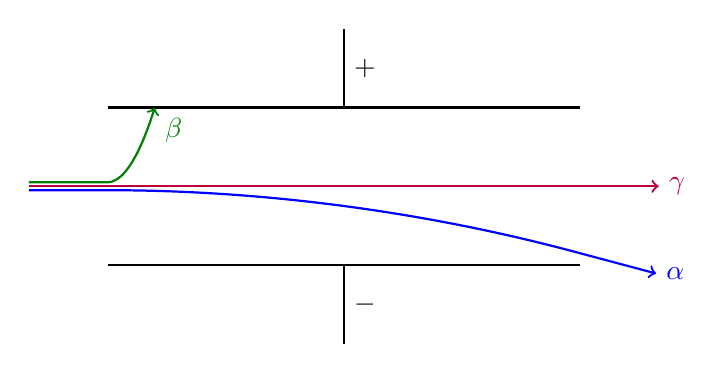
\begin{tikzpicture}
	\draw[thick] (-3,-1) -- (3,-1) (-3,1) -- (3,1);
	\draw[thick] (0,-1) -- (0,-2) node[midway, right] {$-$};
	\draw[thick] (0,1) -- (0,2) node[midway, right] {$+$};
	\draw[thick, purple, ->] (-4,0) -- (4, 0) node[right] {$\gamma$};
	\draw[thick, Green, ->] (-4,0.05) -- (-3,0.05) parabola (-2.4,1) node[below right]{$\beta$};
	\draw[thick, blue, ->] (-4,-0.05) -- (-3,-0.05) parabola (3,-0.85) --++ (-14.93:1) node[right] {$\alpha$};
	\end{tikzpicture}
\end{figure}

\sol $\gamma$-radiation has zero charge, so it is not affected by electric field

$\alpha$-radiation is positively-charged, so it deflects towards the negative plate

$\beta$-radiation is negatively-charged, so it deflects towards the positive plate

$\beta$-particles are much lighter, so they have greater deflection \eoe


\subsubsection*{penetration \& ionising power}

different radiation have different abilities to pass through materials

$\alpha$-, $\beta$- and $\gamma$- radiation are able to knock out orbital electrons from an atom

so radiation can cause the originally neutral atom to become charged

this process is called \keypoint{ionising}\index{ionising power}

\cmt greater ionising ability would imply lower penetration power

radiation loses energy as it passes through a substance

this energy loss is transferred to electrons, causing ionisation of atoms

so the faster radiation gives up its energy, the lower the penetration ability

\cmt $\gamma$-radiation is very penetrative but has very weak ionising power 

$\gamma$-radiation is not charged, and hence it does not interact strongly with electrons

a $\gamma$-photon loses all its energy in single collision and gets absorbed

i.e., one $\gamma$-photon can only ionise one atom

so it has few collisions with electrons, so $\gamma$-radiation is not very ionising

\cmt $\alpha$- and $\beta$-radiation more ionising than $\gamma$-radiation

this is because $\alpha$- and $\beta$-radiation are charged, making them interact with electrons more easily

\cmt $\alpha$-particles are highly ionising

recall $\alpha$-particles are much more massive than electrons

so one $\alpha$-particle can knock out many electrons before it loses all of its kinetic energy

also $\alpha$-particles travel at low speeds, so frequent collision events take place in short range

therefore $\alpha$-radiation has strong ionising ability but weak penetration power

\cmt the table below summarises penetration and ionising power of radioactive radiation

\begin{center}
	\begin{tabular}{|C{3cm}|C{3.2cm}|C{3.2cm}|C{3.2cm}|}
		\hline  & $\alpha$-radiation & $\beta$-radiation & $\gamma$-radiation \\ 
		\hline \multirow{2}{3.2cm}[-20pt]{penetration power} & low & fair & high \\
		 & stopped by thick cardboard or a few centimetres of air & stopped by metal plates of a few millimetres thick & stopped by thick lead or concrete of a few centimetres\\
		\hline ionising power & high & fair & low \\ 
		\hline
	\end{tabular} 
\end{center}



\subsubsection{laws of conservation}

some of the conserved quantities during any decay process are:

\cmt conservation of \emph{electric charge}

\cmt conservation of \emph{charge number} ($Z$)\index{charge number}

this is a consequence of the conservation of electric charge

\cmt conservation of \emph{mass-energy}\index{mass-energy conservation}

Einstein's theory of relativity suggests that mass is equivalent to energy $E=mc^2$

for any naturally occurring nuclear decay process that releases energy, total mass of product particles will be \emph{less} than that of the original particles

reduction in mass becomes of the energy released, which can be kinetic energy of product particles, electromagnetic energy of $\gamma$-radiation emitted, etc.

\cmt conservation of \emph{mass number} ($A$)\index{mass number}

notice that mass number is not exactly proportional to mass of nucleus

mass itself is not conserved during the reaction but only the mass number is conserved

\cmt conservation of \emph{momentum} (review \S\ref{ch:momentum-conservation} if needed)

no external force is involved in nuclear decays, so total momentum is also constant

more specifically, when a stationary nucleus decays into two product particles, for example, the two product particles after an $\alpha$-decay process should move off with equal but opposite momenta


\subsubsection{decay equations}

using nuclide notation, radioactive decay processes can be described by \emph{decay equations}

the conserved quantities provide a simple guideline to write the decay equations 

\begin{compactenum}
	\item[--] sum of charge numbers ($Z$) on both sides of the equation should add up
	
	\item[--] sum of mass numbers ($A$) on both sides of the equation should add up
\end{compactenum}


\example{The first reported nuclear reaction was credited to Ernest Rutherford. By firing $\alpha$-particles into pure nitrogen, Rutherford observed the ejection of hydrogen nuclei from the gas, which is now regarded as the discovery of protons. This reaction can be given by:}
\begin{equation*}
_{\phantom{0}7}^{14} \text{N} + _2^4 \alpha \longrightarrow _{\phantom{0}8}^{17} \text{O} + _{1}^{1} \text{p} \teoe
\end{equation*} 


\example{One reaction that is widely used to power nuclear reactors is the induced fission of uranium-235. The reaction can be triggered by bombarding the uranium-235 nuclei with slow neutrons. The uranium nucleus would split up into two lighter nuclei and release a large amount of energy. One of such reactions can be described by:}
\begin{equation*}
 _{\phantom{0}92}^{235} \text{U} + _0^1 \text{n} \longrightarrow _{\phantom{0}56}^{141} \text{Ba} + _{36}^{92} \text{Kr} + 3_0^1 \text{n} \teoe
\end{equation*} 




\subsubsection*{equation for \texorpdfstring{$\alpha$}{\textalpha}-decays}\index{radioactive decay!$\alpha$-decay}

if a nuclide $_Z^A X$ undergoes $\alpha$-decays, then we have:
\begin{equation*}
\boxed{_Z^A X \longrightarrow _{Z-2}^{A-4} Y + _2^4\alpha}
\end{equation*}

the original nucleus lost two protons and two neutrons during the decay

on both sides of the equation, there are $Z$ protons and $(A-Z)$ neutrons

therefore $\alpha$-decay simply is an $\alpha$-particle escaping from the nucleus



\example{The process in which a uranium-238 nucleus naturally decays into a thorium-234 nucleus through $\alpha$-emission can be written as:}
\begin{equation*}
	_{\phantom{0}92}^{238} \text{U} \longrightarrow _{\phantom{0}90}^{234} \text{Th} + _2^4\alpha \teoe
\end{equation*}



\subsubsection*{equation for \texorpdfstring{$\gamma$}{\textgamma}-decays}\index{radioactive decay!$\gamma$-decay}

$\gamma$-radiation has zero charge and zero mass, so decay equation is very straightforward:
\begin{equation*}
\boxed{_Z^A X \longrightarrow _{Z}^{A} X + _0^0\gamma}
\end{equation*}

since $\gamma$-radiation is pure energy, so there is no change of structure of the nucleus in any way



\subsubsection*{problems with \texorpdfstring{$\beta$}{\textbeta}-decays}\index{radioactive decay!$\beta$-decay}

for $\beta$-decays, one might attempt to write: $
	_Z^A X \longrightarrow _{Z+1}^{\phantom{1+}A} Y + _{-1}^{\phantom{+}0}\beta$ 

on the left, nuclide $X$ has $Z$ protons and $(A-Z)$ neutrons

but on the right, nuclide $Y$ has $(Z+1)$ protons and $(A-Z-1)$ neutrons

one neutron has transformed into a proton through giving off an electron: $_0^1 \text{n} \longrightarrow _1^1 \text{p} + _{-1}^{\phantom{+}0}\text{e} \,\, \text{???}$

but how can neutrons and protons transform into one another?!

further experiments show that $\beta$-particles emitted for same source have \emph{a range of speeds}

this seems to indicate that energy released from a $\beta$-decay can be indefinite

both considerations imply something is wrong, our understanding of $\beta$-decay is not complete

\begin{compactenum}
	\item[--] protons and neutrons cannot be the most fundamental particles of nature
	
	there must exist some more fundamental constituent particles
	
	these are now known as \emph{quarks}, we will discuss them in the next section
	
	\item[--] there must be some other unseen particles released during $\beta$-decays
	
	these particles carry off a fraction of the energy released from the reaction
	
	for conservation laws to hold, they must be chargeless and very light (maybe massless)
	
	these ghostly particles are called \keypoint{neutrinos}, or more precisely, \keypoint{anti-neutrinos}\index{neutrino}
\end{compactenum}

\cmt we thereby can rewrite the $\beta$-decay equation for nuclide $_Z^A X$:
\begin{equation*}
\boxed{_Z^A X \longrightarrow _{Z+1}^{\phantom{1+}A} Y + _{-1}^{\phantom{+}0}\beta + _0^0 \bar{\nu}} \quad \text{or} \quad \boxed{_0^1 \text{n} \longrightarrow _1^1 \text{p} + _{-1}^{\phantom{+}0}\beta + _0^0 \bar{\nu}} \label{eqn:beta-decay}
\end{equation*}

\cmt distribution of kinetic energy of $\beta$-particles can be then explained

only total energy of $\beta$-particle and anti-neutrino is constant

anti-neutrinos also carry some energy, so $\beta$-particles have a range of energies

\example{Radon $^{222}_{\phantom{2}86}\text{Rn}$ decays in a sequence of processes to form bismuth $^{214}_{\phantom{2}83}\text{Bi}$ by emitting $\alpha$-particles and $\beta$-particles. For the decay chain of each radon nucleus, how many $\alpha$-particles and $\beta$-particles are emitted?}

\sol let $x$ be number of $\alpha$-particles emitted and $y$ be number of $\beta$-particles emitted
\begin{equation*}
	^{222}_{\phantom{2}86}\text{Rn} \longrightarrow ^{214}_{\phantom{2}83}\text{Bi} + x \cdot ^4_2 \alpha + y \cdot _{-1}^{\phantom{+}0}\beta + y \cdot _0^0 \bar{\nu}
\end{equation*}

\eqyskip mass number and charge number are conserved: $\Bigg\{$

\vspace*{-1.58\baselineskip}\hspace*{218pt} $\begin{array}{l}
4x + 214 = 222\\[-5pt]
2x - y + 83 = 86
\end{array} \RA x = 2$, $y=1$ \eoe



\subsection{fundamental particles}

In early 20th century, lots of new subatomic particles were discovered in \emph{cosmic rays} and \emph{particle accelerators}. Many of these particles did not fit into the model where proton, neutrons and electrons are the fundamental building blocks for the physical world. To incorporate these subatomic particles discovered at the time, physicist worked out the \keypoint{Standard Model of particle physics}.\footnote{The theory of the Standard Model was developed in stages since the 1950s, through the work of many great scientists, with the current formulation being finalized in the 1970s.\index{Standard Model}
	\begin{compactitem}
		\item[--] \emph{Chen Ning Yang} and \emph{Robert Mills} developed the concept of \emph{gauge theory}, to provide an explanation for the interaction between elementary particles.
		
		\item[--] \emph{Sheldon Glashow} proposed the symmetry group that forms the basis of the accepted \emph{electroweak theory}, in which the electromagnetic interaction and weak interactions are unified into a single force.
		
		\item[--] \emph{Peter Higgs} and two other groups proposed the \emph{Higgs mechanism} that give rise to mass generation for elementary particles without violating gauge theory through a process called \emph{symmetry breaking}.
		
		\item[--] \emph{Steven Weinberg} and \emph{Abdus Salam} incorporated the Higgs mechanism into Glashow's theory, finalizing the unified electroweak theory.
		
		\item[--] \emph{David Gross}, \emph{Frank Wilczek}, \emph{David Politze}, and many others developed \emph{quantum chromodynamics}, the theory of the strong interaction, into its modern form.
		
		\item[--] $\cdots$
	\end{compactitem}

Being the most accurate accurate scientific theory known to human beings, the Standard Model is now regarded as one of the greatest triumphs of modern physics. The theory not only describes the particles known to scientists, but also predicted new particles, including the \emph{Higgs boson}. }


\subsubsection{particles \& anti-particles}

for any particle $\text{p}$, there exists an associated \keypoint{anti-particle} $\bar{\text{p}}$\index{anti-particle}

\cmt an anti-particle has the same mass but opposite charge to its counterpart

\cmt when a particle meets its anti-particle, they \keypoint{annihilate} each other and produce two $\gamma$-photons

combined mass-energy of the pair is converted into electromagnetic energy
\footnote{The energy release from the annihilation of  particle pairs could be potentially used a energy source. The idea of using antimatter to power spaceships or weapons can be found in many science fiction stories.}



\example{Suggest the properties of the anti-particle of the electron.}

\sol anti-particle of electron has same electron mass: $m_e = 9.11\times10^{-31} \text{ kg}$

but it has a positive charge: $q = +e = + 1.60\times10^{-19} \text{ C}$

anti-particle of electron is usually called a \keypoint{positron} (positive electron) with the symbol $\text{e}^+$ \eoe


\subsubsection{quarks \& hadrons}

one type of the elementary matter particle is the \keypoint{quark}\index{quark}

\cmt quarks come in six varieties, or six \keypoint{flavours}

they are \keypoint{up} (u), \keypoint{down} (d), \keypoint{strange} (s), \keypoint{chartm} (c), \keypoint{top} (t), \keypoint{bottom} (b)

\cmt each quark carries an electric charge, as given in the table below

\begin{center}
	{\renewcommand{\arraystretch}{1.35}
		\begin{tabular}{|C{3cm}|C{2cm}|C{2cm}|}
			\hline  & u & d \\
			 quarks & c & s \\
			  & t & b \\
			\hline charge & $+\frac{2}{3}e$ & $-\frac{1}{3}e$ \\[3pt]
			\hline
		\end{tabular}
	}
\end{center}

note that all quarks carry a \emph{fraction} of the elementary charge unit\footnote{Each horizontal line in the table is known as a \emph{generations} of quarks. As you can see, there are three generations of quarks.}

\cmt quarks can combine to form composite particles called \keypoint{hadrons} \index{hadron}

there are two ways that several quarks can make up a hadron

\begin{compactenum}
	\item[--] hadrons can be made up of three quarks (qqq), called \keypoint{baryons} \index{baryon}
	
	members of the baryon family include protons and neutrons
	
	a proton consists of two up quarks and one down quark (uud) \index{proton}
	
	a neutron consists of one up quark and two down quarks (udd) \index{neutron}
	
	\item[--] hadrons can also be made up of one quark and one anti-quark (q$\bar{\text{q}}$), called \keypoint{mesons} \index{meson}
	
	you don't need to memorise any example of meson
	
	you are only required to identify if a particle is a meson given the quark composition
\end{compactenum}

\cmt quarks and hadrons are affected by the \keypoint{strong nuclear force}\index{strong nuclear force}

strong nuclear force is a very short-ranged attractive force

\begin{compactenum}
	\item[--] it is responsible for hold quarks close together to from hadrons

	\item[--] it is also responsible for the attraction between hadrons
	
	for example, protons and neutrons are held together in a nucleus by strong force
	\footnote{For a small nucleus, strength of strong nuclear force is way greater than the electric repulsion between positively-charged protons, hence the force bind protons and neutrons together forming a stable nucleus. However, since the strong nuclear force has a very short range, the repulsive electrostatic force between the protons might dominate the attractive nuclear force for an over-sized nucleus. Such large nuclei become unstable and are likely to undergo \emph{radioactive decays}.}
\end{compactenum}


\cmt quarks only exist in hadrons, i.e., there are no single free quarks in nature\footnote{This is known as the \emph{confinement}, a consequence that is closely related to the fact that interaction between quarks are weak at high energies or smaller length scales but strong at low energies or large length scales, a feature of strong nuclear forces known as \emph{asymptotic freedom}.}


\example{By reference to the quark composition, explain the electric charge of protons and neutrons.}

\sol charge of proton (uud): $q_\text{p} = 2q_\text{u} + q_\text{d} = 2\times\left(+\frac{2}{3}e\right) + \left(-\frac{1}{3}e\right) = +e$

\eqyskip charge of neutron (udd): $q_\text{n} = q_\text{u} + 2q_\text{d} = \left(+\frac{2}{3}e\right) + 2\times\left(-\frac{1}{3}e\right) = 0$ \eoe

\example{A meson has an electric charge of $+e$ and is known to contain an up quark. Determine a possible flavour of the other quark.}

\sol charge of the other quark is: $(+e) - \left(+\frac{2}{3}e\right) = +\frac{1}{3}e$

this could be an anti-down ($\bar{\text{d}}$), an anti-strange ($\bar{\text{s}}$), or an anti-bottom quark ($\bar{\text{b}}$)\eoe



\subsubsection{leptons}

another type of the elementary matter particle is the \keypoint{lepton}\index{lepton}

\cmt leptons are not affected by strong nuclear forces

\cmt members of the lepton family include electrons (e), neutrinos ($\nu$), muons ($\mu$), taons ($\tau$)\footnote{Just like the quarks, leptons also come in three \emph{generations}. Each generation of leptons consists of an electron-like particle and its associated neutrino.}

in A-Level exams, you only need to know electrons (e) and neutrinos ($\nu$)


\cmt for each particle, one can assign a \keypoint{lepton number} $L$

\begin{compactitem}
	\item[--] a lepton has lepton number $L=+1$
	
	\item[--] an anti-lepton has lepton number $L=-1$
	
	 \item[--]any other particle has lepton number $L=0$
\end{compactitem}

classification of sub-atomic particles within the A-Level syllabus\footnote{This is an over-simplified version of the Standard Model. I only included the particles that you need to know for the A-Level exams. There are a lot of missing pieces that are way beyond the scope of our course, so please don't take this mindmap too seriously.} is summarised below

\begin{figure}[ht]
	\centering
	\begin{tikzpicture}
%	\draw[help lines, gray!30, step=0.5] (0,-5) grid (15,5);
%	\foreach \x in {1,2,...,15} \node[below] at (\x,0) {\x};
%	\foreach \y in {-5,-4,...,5} \node[left] at (0,\y) {\y};
	% root / fundamental particles
	\draw (2.5,0.4) -- (3.5,0.4) (4.5, -1.7) -- (3.5,-1.7) -- (3.5, 2.5) -- (4.5, 2.5);
	\draw[rounded corners, fill=white] (0.1,-0.3) rectangle (2.5,1.1);
	\draw (1.3,0.4) node[twolinecap] {fundamental\\particles};
	% quarks
	\draw[rounded corners, fill=white] (4.3,2.2) rectangle (5.9, 2.8);
	\draw (5.1, 2.5) node {quarks};	
	\draw (5.0, 2.1) -- (4.6, 1.6);
	\draw (5.2, 2.1) -- (5.6, 1.6);
	\node at (4.6, 1.4) {u};
	\node at (5.6, 1.4) {d};
	\node at (4.6, 0.9) {c};
	\node at (5.6, 0.9) {s};
	\node at (4.6, 0.4) {t};
	\node at (5.6, 0.4) {b};
	\node at (4.6, -0.2) {{\scriptsize $+\frac{2}{3}e$}};
	\node at (5.6, -0.2) {{\scriptsize $-\frac{1}{3}e$}};
	% leptons
	\draw[rounded corners, fill=white] (4.3,-1.4) rectangle (5.9, -2.0);
	\draw (5.1, -1.7) node {leptons};
	\draw (5.0, -2.1) -- (4.6, -2.6) node[below]{e};
	\draw (5.2, -2.1) -- (5.6, -2.6) node[below]{$\nu$};
	\node at (4.6, -3.2) {{\scriptsize $-e$}};
	\node at (5.6, -3.2) {{\scriptsize $0$}};
	% hadrons
	\draw[dashed, ->] (5.9, 2.5) -- (8.1,2.5) node[midway, above]{make up};
	\draw[rounded corners, fill=white] (8.1,2.2) rectangle (9.9, 2.8);
	\draw (9, 2.5) node {hadrons};
	% baryons
	\draw (9.9, 2.5) -- (10.5, 2.5) -- (10.5, 3.5) -- (12, 3.5) node[midway, above]{(qqq)};
	\draw[rounded corners, fill=white] (12,3.2) rectangle (13.8, 3.8);
	\draw (12.9, 3.5) node {baryons};
	\draw (12.8, 3.1) -- (12.4, 2.6) node[below]{p};
	\draw (13.0, 3.1) -- (13.4, 2.6) node[below]{n};
	% mesons
	\draw (10.5, 2.5) -- (10.5, 1.5) -- (12, 1.5) node[midway, above]{(q$\bar{\text{q}}$)};
	\draw[rounded corners, fill=white] (12,1.2) rectangle (13.8, 1.8);
	\draw (12.9, 1.5) node {mesons};
	\end{tikzpicture}
	\caption*{a coarse guide for classifying sub-atomic particles in A-Level physics}
\end{figure}



\subsubsection{\texorpdfstring{$\beta$}{\textbeta}-decays}\index{radioactive decay!$\beta$-decay}

there exists positron, anti-particle of electron, so there are two types of $\beta$-particles: $\beta^-$ and $\beta^+$

hence two types of $\beta$-decays are possible: $\beta^-$-decay and $\beta^+$-decay



\subsubsection*{\texorpdfstring{$\beta^-$}{\textbeta\textsubscript{-}}-decay revisited}

a neutron changes into a proton during a $\beta^-$-decay: $\boxed{_0^1 \text{n} \longrightarrow _1^1 \text{p} + _{-1}^{\phantom{+}0}\beta + _0^0 \bar{\nu}} $

we have learned about the quark structures of protons (uud) and neutrons (udd)

therefore $\beta^-$-decay process at a more fundamental level is: $ \boxed{\text{d} \longrightarrow \text{u} + \beta^- + \bar{\nu}} $


\subsubsection*{\texorpdfstring{$\beta^+$}{\textbeta\textsubscript{+}}-decay}


$\beta^+$-decay occurs when a proton changes into a neutron and emits a positron

$\beta^+$-decay process is described by the equation: $ \boxed{_1^1 \text{p} \longrightarrow _0^1 \text{n} + _{+1}^{\phantom{+}0}\beta + _0^0 \nu} $

in terms of quarks, $\beta^+$-decay can be rewritten as: $ \boxed{\text{u} \longrightarrow \text{d} + \beta^+ + \nu} $

\cmt nature of $\beta$-decay processes is the transformation of quark flavours

the interaction responsible for this transformation is the \keypoint{weak nuclear force}\index{weak nuclear force}

\cmt there is yet another law of conservation -- the \keypoint{conservation of lepton number}

we can use lepton number to predict whether a neutrino or an anti-neutrino is emitted

\example{Verify the conservation of (a) charge number, (b) mass number, and (c) lepton number for the $\beta^+$-decay process: $_1^1 \text{p} \longrightarrow _0^1 \text{n} + _{+1}^{\phantom{+}0}\beta + _0^0 \nu$}

\sol charge number conservation: $+1 = 0 + (+1) + 0$ \xskip \ding{51}

mass number conservation: $1 = 1 + 0 + 0$ \xskip \ding{51}

lepton number conservation: $0 = 0 + (-1) + (+1)$ \xskip \ding{51}

so this reaction does not violate any of these conservation law \eoe


\example{\emph{Electron capture} is a process where an electron in an atom's inner shell is drawn into the nucleus and combines with a proton. The result is to form a neutron and a neutrino. The process can be given by: $_1^1 \text{p} + _{-1}^{\phantom{+}0}\text{e} \longrightarrow _0^1 \text{n} +  + _0^0 \nu$. Show that the process satisfies the conservation of (a) charge number, (b) mass number, and (c) lepton number.}

\sol charge number conservation: $+1 + (-1) = 0 + 0$  \xskip \ding{51}

mass number conservation: $1 + 0 = 1 + 0$ \xskip \ding{51}

lepton number conservation: $0 + 1 = 0 + 1$  \xskip \ding{51}

so this reaction does not violate any of these conservation law \eoe


\ifthenelse{\includequestions=1}{
	
\subsection{end-of-chapter questions}

\subsection*{atomic structure}

\question{
	List the number of sub-atomic particles in an argon-40 ($^{40}_{18}\text{Ar}$) atom.
}






\subsection*{radioactive decays}
	
\question{
	A radioactive source emits a parallel beam of $\alpha$-, $\beta$- and $\gamma$-radiation. A detector sensitive to all forms of radiation has been calibrated for background radiation and is placed just 1 cm from the radioactive source. The detector registers 500 counts s$^{-1}$.  
		
	When the detector is 10 cm from the source, the radiation level drops to 200 counts s$^{-1}$.
	
	When a thin aluminium sheet is placed in front of the detector, the level falls to 50 counts s$^{-1}$.
	
	In what proportion is the source emitting $\alpha$-, $\beta$- and $\gamma$-particles?
}



\subsection*{nuclear equations}

\question{
	An unstable isotope of phosphorus, $_{15}^{30}$P can be produced by bombarding aluminium, $_{13}^{27}$Al, with $\alpha$-particles. What is the by-product of this reaction?
}

\question{
	Carbon-14 ($^{14}_{\phantom{0}6}$ C) undergoes $\beta$-decay and forms an isotope of nitrogen (N). Write down the decay equation using the nuclide notations.
}

\question{
	Radon-222 ($^{222}_{\phantom{2}86}$Rn) undergoes a series of decays and forms lead-210 ($^{210}_{\phantom{2}82}$Pb). 
	How many $\alpha$-particles and $\beta$-particle are emitted during this process?
}

\subsection*{fundamental particles}


\question{
	State the mass and electric charge of an anti-proton.
}

\question{
	$\pi^+$ is a particle with quark structure $u\bar{d}$. (a) State the family of this particle. (b) Show that it carries a charge of $+e$. (c) Suggest the charge of its anti-particle.
}



\question{
	$\Xi^0$ is a particle with quark structure $uss$. (a) State the family of $\Xi^0$. (b) Find its electric charge.
}

\question{
	Magnesium-23 ($^{23}_{12}$Mg) can decay into sodium-23 ($^{23}_{11}$Na). (a) Write down the decay equation using nuclide notation, and specify any other product particles produced. (b) Write an equation for this decay in terms of protons and neutrons. (c) Write an equation for this decay in terms of quark composition. (d) State the name of the force that is responsible for this decay.
}
	
}{}

